\section{Anwendungen}

\subsection{Objektlageerkennung in Tiefendaten} 

\subsubsection{Ausgangslage}
In der Schmiede- und Giessereibranche ist das Handling der häufig schweren und unhandlichen Werkstücke mittels Robotern eine grosse Herausforderung. Eine der Grundvoraussetzungen ist dabei auch eine hohe Flexibilität, um häufige Produktwechsel behandeln zu können. Ein bekanntes Problem ist der sogenannte "Griff-in-die-Kiste", d.h. die Entnahme eines bestimmten Gegenstandes aus einer mit mehreren chaotisch angeordneten Objekten gefüllten Kiste. \\

Die Dissertation \cite{Diss-Ledermann} von Thomas Ledermann beschäftigt sich u.a. mit der Entnahme von Getriebewellen für eine Ultraschallprüfung zur automatischen Qualitätssicherung. Dabei stellt sich zum Beispiel folgende Ausgangslage: \\

\begin{figure}[htbp]
	\centering
	\begin{minipage}{6cm}
		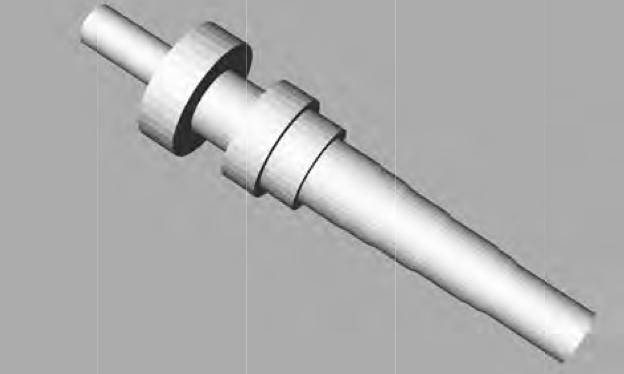
\includegraphics[width=5cm]{images/welle-cad}
	\end{minipage}
	\begin{minipage}{6cm}
		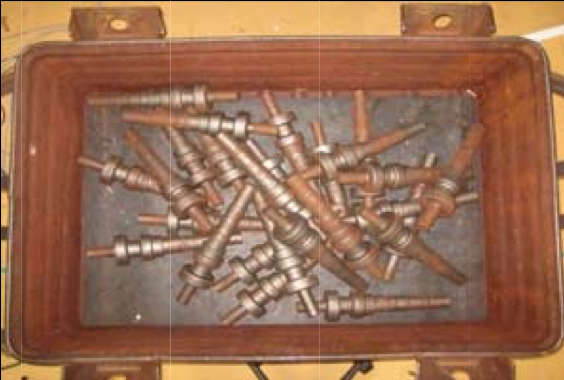
\includegraphics[width=5cm]{images/welle-kiste}
	\end{minipage}
	\caption{	Links: CAD-Modell einer Getriebewelle \\
				Rechts: Beispiel einer Kiste mit Getriebewellen zur Ultraschallprüfung}
	\label{Fig-Getriebewelle}
\end{figure}

Es müssen nebst den Getriebewellen auch verschiedene weitere Objekte, wie Hohlringe oder Gehäusedeckel erkennbar sein. Für alle Gegenstände werden die entsprechenden 3D-CAD-Daten geliefert. Die Objekte liegen immer artenrein vor, d.h. es kommt immer nur eine Art Teile vor. \\

\subsubsection{Umsetzung}
Zur Erkennung der Objekte muss eine Wissensbasis $W$ bestehend aus Merkmalen des Objekts bekannt sein. Gut auswertbar sind in erster Linie Merkmale, wie Kreise / Ellipsen, Kantenzüge, Ebenen, Volumenkörper, Histogramme. Alle diese Merkmale bis auf Histogramme schränken die Objektbeschreibung stark ein, weil nicht alle Objekte über solche Merkmale verfügen. Als beste Wahl herausgestellt hat sich deshalb die Verwendung von Histogrammen. \\

Für die gegebenen Tiefendaten $T = \{ (x,y,z) \in \mathbb{R}^3 ; T(x,y)=z\}$ werden folgende Auswertungen gemacht: \\

\textbf{Objektorientierung $R_i$}: Die Objektorientierung gibt an, mit welchem Eintrag aus der Wissensbasis die Partikelposition verglichen werden soll. Zur Bestimmung der Orientierung gibt es verschiedene Ansätze. Gegenüber der Darstellung mittels Richtungskosinus oder Quaternionen hat sich aufgrund der Einfachheit und der Anschaulichkeit die in der Luftfahrt verbreitete Yaw-Pitch-Roll-Variante der Eulerwinkel durchgesetzt.

\begin{figure}[htbp]
	\centering
	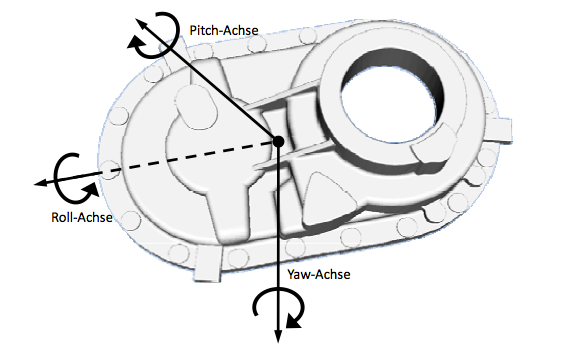
\includegraphics[width=6cm]{images/yaw-pitch-roll}
	\caption{Yaw-Pitch-Roll-Variante der Eulerwinkel}
	\label{Fig-Yaw-Pitch-Roll}
\end{figure}

\textbf{Objektposition $P_i$}: Die Objektposition gibt an, an welcher Stelle der Tiefendaten der Vergleich stattfinden soll. Als Referenzpunkt für die Position ist der höchste Punkt des Objekts am besten geeignet, weil dieser einfach aus den Tiefendaten extrahierbar ist. \\

\textbf{Objektmerkmalsdaten $C_i$}: Die Objektmerkmalsdaten geben an, welche Tiefendaten ausgehend von $P_i$ in die Auswertung einbezogen werden sollen. Sämtliche Tiefenwerte, welche zur potentiellen Objektlage gehören, müssen mittels einer geeigneten Segmentierung vom Hintergrund getrennt werden. \\

Mathematisch sind die Positionsdaten und die Fitnessfunktion also folgendermassen definiert: 
\begin{align}
	p_i &= f(\alpha ,\beta ,\gamma) \\
	f(p_i) &= f(R_i,P_i,C_i)
\end{align}

\subsubsection{Resultate}
Der Partikelschwarm wird mit 100 Partikeln in lbest Topologie mit 30 Nachbarn realisiert. Bei 100 Iterationen wird innerhalb von 4 Sekunden ein Resultat erreicht. In einer Kiste mit 50 Teilen wurden lediglich 4 Objektpositionen falsch erkannt, was einer Erkennungsrate von 92 \% entspricht. Nach erneutem scannen werden auch die falsch erkannten Teile meist korrekt erkannt. Weitere Verbesserungen zur Verkürzung der Taktzeiten und zur gleichzeitigen Erkennung  mehrerer Objekte sind in Planung und sollten gut realisierbar sein.

\subsection{Analyse neuraler Netzwerke}
Ein weiteres Anwendungsgebiet, in welchem die Partikelschwarm Optimierung erfolgreich eingesetzt wird, ist die Analyse neuraler Netzwerke , u.a. in der Medizin. Eine übliche Anwendung ist bei der Diagnose von Parkinson und Tremor zu finden. Dabei werden Bewegungsdaten von einem Aktigraph-System (Messung der Bewegung, sowie der Umgebungstemperatur und -Helligkeit ) werden verarbeitet um zwischen \textacutedbl normalen\textacutedbl \ und von Krankheit verursachten Bewegungen zu unterscheiden. \cite{Shi-Appl}

\subsection{Zucht von Mikroorganismen}
Eine grosse Herausforderung in der Zucht von Mikroorganismen ist die ideale Zusammensetzung der Nährstoffe. Die Verwendung der PSO hat sich in diesem Bereich stark durchgesetzt. Gegenüber klassischer Optimierungen hat die PSO komplett andere Mischungen herausgebracht, welche sich als bis zu doppelt so wirksam erwiesen haben. \cite{Shi-Appl}